\documentclass[12pt,a4paper]{article}
\usepackage[utf8]{inputenc}
\usepackage[german]{babel}
\usepackage[T1]{fontenc}
\usepackage{amsmath}
\usepackage{amsfonts}
\usepackage{amssymb}
\usepackage{graphicx}
\usepackage{siunitx}
\usepackage[left=2cm,right=2cm,top=2cm,bottom=2cm]{geometry}
\author{Tim}

\begin{document}
	\setlength{\parindent}{0pt} 
	\begin{center}
		{\LARGE Versuchsprotokoll}\\
		\begin{large}
			zum Grundpraktikum Physik Teil II\\[0.4cm]
			an der RWTH Aachen\\
			I. Physikalisches Institut B\\[4.5cm]
			\Large\textbf{\textsl{Atomphysik}}\\[4cm]
			\normalsize\textit{vorgelegt\\von}\\[0.4cm]
			\large{Moritz Berger\\Tim Herbermann\\Gerald Kolter\\Sebastian Siebert}\\[1cm]
			\large \textit{Gruppe A07} \\ [3cm]
			\large \textbf{Sommersemester 2017}
		\end{large}
	\end{center}
	\newpage
	
\tableofcontents
\newpage

\section{Versuchsziele}
In diesem Versuch soll durch Vermessung der sogenannte Wärmestrahlung eines Lesliewürfels das Stefan-Boltzmann Gesetz nachgewiesen werden. Dabei sollen die Emissionskoeffizienten von 4 Seiten des Würfels bestimmt werden.

\section{Physikalische Grundlagen}
Jeder Körper hat eine Temperatur größer als \SI{0}{K} und sendet elektromagnetische Strahlung aus; diese wird Temperaturstrahlung oder auch Wärmestrahlung genannt. \\
Der Wärmeaustausch zwischen zwei Körpern kann auf 3 verschiedene Arten geschehen:
\begin{enumerate}
\item Konvektion: Der Austausch von Wärmeenergie durch Austausch von Teilchen
\item Wärmeleitung: Der Austausch von Wärmeenergie zwischen zwei einander berührende Körpern
\item Wärmestrahlung: Der Austausch von Wärmeenergie durch Abstrahlen von elektromagnetischer Strahlung bei einem der Körper und Absorption der Strahlung durch den anderen Körper
\end{enumerate}
Es soll in diesem Versuch nur um die Wärmestrahlung gehen, daher muss darauf geachtet werden, dass Konvektion und insbesondere Wärmeleitung verhindert wird. \\
Die Wärmestrahlung bildet ein kontinuierliches Spektrum. 

\paragraph{Das Plancksche Strahlungsgesetz}\mbox{}\\
Für das Emissionsvermögen eines schwarzen Körpers wurde um 1900 von Max Planck ein Modell vorgeschlagen, das die Quantenmechanik mitbegründet hat. Entscheidend hierbei ist, dass die elektromagnetische Wechselwirkung mit dem schwarzen Körper gequantelt ist; der Austausch von Energie mit dem Strahlungsfeld kann nur mit Vielfachen der Photonenenergie $E_\gamma = h \cdot f$ stattfinden. Für das Emissionsvermögen eines schwarzen Körpers ergibt sich das Plancksche Strahlungsgesetz zu:
\begin{equation}
E_{\lambda, s} = 2 \pi \cdot \dfrac{h c^2}{\lambda^5} \cdot \dfrac{1}{e^{\frac{hc}{\lambda kT}} - 1}
\end{equation}
Integriert man dieses Emissionsvermögen über alle Wellenlängen, erhält man die gesamte abgestrahlte Leistung:
\begin{equation}
P = E_s (T) = \int_0^\infty E_{\lambda, s} (\lambda, T) d\lambda = \sigma T^4 \qquad mit \qquad \sigma = \dfrac{2 \pi^5 k^4}{15h^3c^2}
\label{Stefan_Boltzmann_Gesetz_schwarz}
\end{equation}
Für einen nicht-schwarzen Körper (also mit Emissionskoeffizient $\varepsilon \neq$ 1) muss Gl. \ref{Stefan_Boltzmann_Gesetz_schwarz} modifiziert werden. Dabei werden in diesem Versuch zur Vereinfachung nur graue Körper betrachtet, das bedeutet, dass der Emissionskoeffizient $\varepsilon$ über die Wellenlänge konstant ist. Das Stefan-Boltzmann Gesetz sieht für solche Körper dann wie folgt aus:
\begin{equation}
P = \varepsilon \sigma T^4 \qquad mit \qquad \sigma = \dfrac{2 \pi^5 k^4}{15h^3c^2}
\label{Stefan_Boltzmann_Gesetz_grau}
\end{equation}
Wichtig für die Auswertung ist, dass der Versuch in Luft bei Umgebungsdruck und Zimmertemperatur durchgeführt wurde. Die Umgebung strahlt ebenfalls auf den Körper, sodass die letztlich gemessene Strahlungsleistung die Differenz zwischen der Strahlung des Körpers und der Strahlung der Umgebung ist:
\begin{equation}
P = \varepsilon \sigma (T^4 - T_0^4)
\label{Stefan_Boltzmann_Gesetz_gemessen}
\end{equation}
Mit der Umgebungstemperatur $T_0$.



\section{Aufbau und Durchführung}
\subsection{Aufbau}
\begin{figure}
\centering
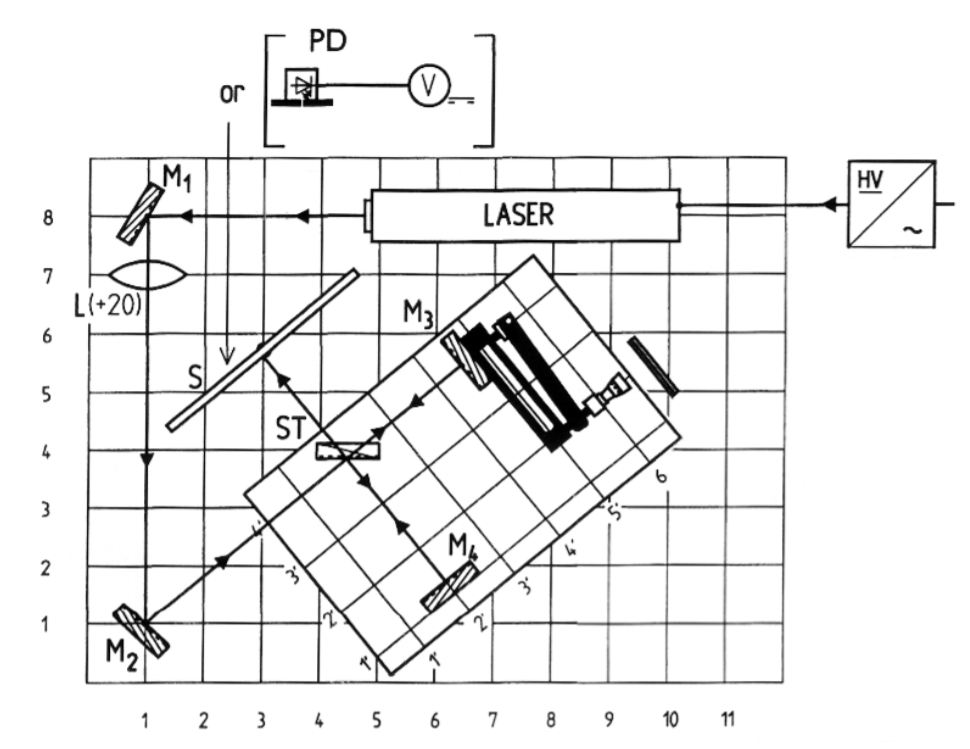
\includegraphics[scale=0.6]{Bilder/Aufbau.png}
\caption{Aufbau zur Vermessung der abgestrahlten Leistung einer der Seiten des Lesliewürfels. Die Nummerierung wird im Text erklärt.}
\label{fig:Aufbau}
\end{figure}

Abbildung \ref{fig:Aufbau} zeigt den Aufbau zur Vermessung der abgestrahlten Leistung einer der Seiten des Lesliewürfels.\\
Der Lesliewürfel (3) ist ein Würfel, der mit Wasser gefüllt auf einer Heizplatte (5) steht und 4 verschiedene Seiten hat. Zur besseren Wärmeverteilung im Wasser und damit im Würfel wird ein sogenannter Rührfisch verwendet; dies ist ein kleiner, stabförmiger Magnet, der von einem rotierenden Magneten unterhalb der Heizplatte gedreht wird und damit das Wasser umrührt. Die Temperatur des Wassers wird mit einem an das CASSY (6) angeschlossenen Thermometer gemessen. Die Strahlung wird mit einer Thermosäule nach Moll (2) gemessen. Diese befindet sich auf einer Schiene (1), die der Säule eine gewisse Stabilität gibt und erlaubt, die Thermosäule zwischendurch von dem Würfel zu entfernen, sodass sich das Schutzrohr nicht aufheizt. Da die Thermosäule nur sehr geringe Spannungen liefert, wird zwischen diese und das CASSY ein Verstärker (4) geschaltet.

\subsection{Durchführung}

\section{Auswertung}
\subsection{Gruppe A}
\subsection{Gruppe B}

\section{Anhang}
\subsection{Gruppe A}
\subsection{Gruppe B}
	
\end{document}